\section{Reagenti}
Indica il tipo e le caratteristiche dei reagenti  impiegati (è essenziale segnalare la concentrazione delle soluzioni e, per i solidi, il grado di purezza). A questo scopo ti mostro anche come mettere le euqazioni e formule chimiche con un pacchetto apposito:
\begin{itemize}
    \item \ce{H3PO4} 0.3 M 25 mL
\end{itemize}

\begin{table}[!ht]
    \scriptsize
    \centering
    \begin{tabularx}{1\textwidth}{m{0.15\textwidth}|m{0.2\textwidth}|m{0.23\textwidth}|m{0.17\textwidth}|m{0.13\textwidth}}
        \toprule
        \textbf{Composto} &  \textbf{Formula di struttura} & \textbf{Frasi H e P} & \textbf{Pittogrammi} & \textbf{DPI}\\
        \midrule
        \ce{H2O2}& \begin{center}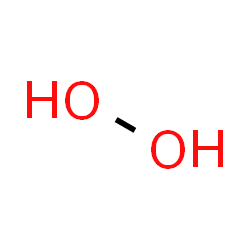
\includegraphics[width=3cm,scale=0.4]{img/763.png} \end{center} & 
             H: H271, H302, H314 e H332.
             
             P: P210, P220, P221, P260, P261, P264, P270, P271, P280, P283, P301+P312, P301+P330+P331, P303+P361+P353, P304+P312, P304+P340, P305+P351+P338, P306+P360, P310, P312, P321, P330, P363, P370+P378, P371+P380+P375, P405, e P501. & \begin{center} \begin{tabular}{cc}
                  
\includegraphics[scale=0.15]{img/pittogrammi/Flammable.png}&  
\includegraphics[scale=0.15]{img/pittogrammi/Explosive.png} \\
                  
\includegraphics[scale=0.15]{img/pittogrammi/Flammable.png}&  
\includegraphics[scale=0.15]{img/pittogrammi/Explosive.png} 
             \end{tabular}\end{center} & guanti, occhiali e visiera\\
    \bottomrule
    \end{tabularx}
    \caption{Tabella con i composti chimici utilizzati nell'esperienza, le frasi P e H vengono riportate per esteso al fondo della relazione.}
    \label{tab:tab1}
    \normalsize
\end{table}





Per i DPI sei costretto a cercare il nome del composto e scrivere di seguito scheda di sicurezza (es. acido benzoico scheda di sicurezza). Cerca di ricordarti il produttore, fai magari una foto in lab del contenitore, perchè possono variare. In fondo alla secheda trovi ache le info sui DPI oltre a altre varie info utili.

Altri siti utili che puoi utilizzare sono:
\begingroup
\begin{multicols}{2}
\begin{itemize}
    \item \href{https://molview.org/}{\textcolor{blue}{MolView}: sito ottimo per avere immagini 2D e 3D dei composti chimici;}
    \item \href{https://echa.europa.eu/it/regulations/clp/clp-pictograms}{\textcolor{blue}{ECHA}: per i simboli dei pittogrammi aiutati con questo se serve;}
    \item \href{https://echa.europa.eu/it/information-on-chemicals/cl-inventory-database}{\textcolor{blue}{ECHA}: per quanto riguarda le informazioni dei composti e la loro classificazione in europa;}
    \item \href{https://pubchem.ncbi.nlm.nih.gov/}{\textcolor{blue}{PubChem}: ottimo sito per informazioni generali dei composti chimici;}
    \item \href{http://www.chemspider.com/}{\textcolor{blue}{ChemSpider}: sito simile a PubChem;}
    \item \href{https://go.drugbank.com/}{\textcolor{blue}{DrugBank}}
    \item \href{https://www.ebi.ac.uk/chebi/init.do}{\textcolor{blue}{Chemical Entities of Biological Interest (ChEBI)}}
    \item \href{https://www.ebi.ac.uk/chembl/}{\textcolor{blue}{ChEMBL Database}}
    \item \href{https://commonchemistry.cas.org/}{\textcolor{blue}{CAS Common Chemistry}}
    \item \href{https://dguv.de/corona/index.jsp}{\textcolor{blue}{DGUV}}
    \item \href{https://www.rcsb.org/}{\textcolor{blue}{RCSB PDB}: Proteine DataBank}
    \item \href{https://www.efsa.europa.eu/it}{\textcolor{blue}{EFSA}: European Food Safety Authority}
    \item \href{http://eawag-bbd.ethz.ch/}{\textcolor{blue}{EAWAG BBD/PPS}: Biocatalysis/Biodegradation Database;}
    \item \href{https://sinu.it/}{\textcolor{blue}{SINU}: Società Italiana di Nutrizione;}
    \item \href{https://www.ars.usda.gov/}{\textcolor{blue}{ARS}: Agricultural Research Service;}
    \item \href{https://www.nist.gov/}{\textcolor{blue}{NIST}: National Istitute of Standards and Technology;}
    \item \href{https://www.rsc.org/merck-index}{\textcolor{blue}{The Merck Index Online}: For over 120 years The Merck Index has been regarded as the most authoritative and reliable source of information on chemicals, drugs and biologicals..}
\end{itemize}
\end{multicols}
\endgroup